\documentclass[12pt, a4paper]{article}

% Codificacao e idioma
\usepackage[utf8]{inputenc}
\usepackage[T1]{fontenc}
\usepackage[brazil]{babel}

% Layout e margem ABNT
\usepackage[top=3cm, bottom=2cm, left=3cm, right=2cm]{geometry}

% Tipografia
\usepackage{times}
\usepackage{setspace}
\onehalfspacing

% Figuras e tabelas
\usepackage{graphicx}
\usepackage{float}
\usepackage{booktabs}
\usepackage{longtable}
\usepackage{array}

% Codigos
\usepackage{listings}
\usepackage{xcolor}

% Links e referencias
\usepackage[hidelinks]{hyperref}
\usepackage[
  backend=biber,
  style=abnt,
  citestyle=abnt
]{biblatex}
\addbibresource{referencias.bib}

% Identacao do primeiro paragrafo
\usepackage{indentfirst}

% Titulos de secao
\setcounter{secnumdepth}{3}
\setcounter{tocdepth}{3}

% Configuracao de listings
\lstset{
  basicstyle=\ttfamily\small,
  breaklines=true,
  frame=single,
  backgroundcolor=\color{gray!10},
  captionpos=b
}

% -----------------------------------------------------------
\begin{document}

% -----------------------------------------------------------
% CAPA
% -----------------------------------------------------------
\begin{titlepage}
\newgeometry{top=2cm, bottom=2cm, left=2.5cm, right=2.5cm}

% Brasao no canto superior esquerdo
\noindent
\begin{minipage}[t]{0.18\textwidth}
  
\includegraphics[height=2.8cm]{figuras/brasao-unisantos.png}
\end{minipage}%
\begin{minipage}[t]{0.82\textwidth}
  \centering
  \vspace{0.3cm}
  {\large\bfseries UNIVERSIDADE CAT\'OLICA DE SANTOS}\\[0.25cm]
  {\large Ci\^encia da Computa\c{c}\~ao}
\end{minipage}

\vfill

% Titulo centralizado
\begin{center}
  {\fontsize{28}{34}\selectfont\bfseries Explora+}\\[0.8cm]
  {\large\bfseries Entrega de Prot\'otipo}
\end{center}

\vfill\vfill

% Autores alinhados a esquerda
\begin{flushleft}
{\large
  Felipe Barbosa dos Santos\\[0.3cm]
  Felipe de Lima Monteiro\\[0.3cm]
  Lucas Carmona Neto\\[0.3cm]
  Lucas Cerqueira Galv\~ao\\[0.3cm]
  Jo\~ao Gabriel Henriques Cardoso
}
\end{flushleft}

\vspace{1.8cm}

% Data centralizada no rodape
\begin{center}
  {\large Santos -- SP, junho de 2026}
\end{center}

\restoregeometry
\end{titlepage}

\thispagestyle{empty}
\tableofcontents
\newpage

% -----------------------------------------------------------
\section{Introdu\c{c}\~ao}
% -----------------------------------------------------------

O projeto Explora+ \'e uma iniciativa de extens\~ao desenvolvida por estudantes de Ci\^encia da Computa\c{c}\~ao da Universidade Cat\'olica de Santos com o objetivo de criar um aplicativo m\'ovel para promo\c{c}\~ao do turismo local.

\subsection{Problema}

Cidades de m\'edio porte como Santos -- SP possuem rico acervo tur\'istico e cultural, mas enfrentam baixa visibilidade de seus atrativos pela aus\^encia de ferramentas digitais acess\'iveis e integradas. Visitantes e moradores frequentemente desconhecem monumentos hist\'oricos, parques e pontos de interesse pr\'oximos, e n\~ao t\^em como planejar percursos tur\'isticos de forma autom\'atica.

\subsection{Solu\c{c}\~ao proposta}

O Explora+ oferece um planejador de rotas tur\'isticas que:

\begin{itemize}
  \item Calcula automaticamente um percurso pedestre entre dois pontos;
  \item Identifica pontos de interesse (POIs) pr\'oximos ao trajeto via dados abertos do OpenStreetMap;
  \item Enriquece os detalhes de cada POI com imagens e resumos buscados no Wikidata e Wikipedia;
  \item Permite ao usu\'ario marcar lugares como visitados, excluir paradas e manter uma biblioteca pessoal de lugares.
\end{itemize}

\subsection{Stakeholder externo}

O cliente externo do projeto \'e Felipe Pacheco Fernandes, CRO do Grupo Costa Norte de Comunica\c{c}\~ao, sediado na Baixada Santista/SP. O grupo atua como stakeholder, contribuindo com feedback sobre comunica\c{c}\~ao e facilitando contato com estabelecimentos comerciais e ag\^encias de turismo locais.

% -----------------------------------------------------------
\section{Desenvolvimento}
% -----------------------------------------------------------

\subsection{Metodologia e organiza\c{c}\~ao do time}

O time adotou metodologia \'agil com sprints semanais, organiza\c{c}\~ao de tarefas via Trello e reuni\~oes peri\'odicas com o Product Owner externo. O reposit\'orio foi estruturado em tr\^es projetos independentes:

\begin{itemize}
  \item \texttt{explora-plus-backend} -- API Django;
  \item \texttt{explora-plus-frontend} -- app Expo/React Native;
  \item \texttt{explora-plus-docs} -- documenta\c{c}\~ao, modelagem e paper.
\end{itemize}

\subsection{Proposta inicial de arquitetura}

No in\'icio do semestre, a arquitetura proposta previa integra\c{c}\~ao com APIs comerciais como Google Maps (geolocaliza\c{c}\~ao e roteamento), GeoAPIFy (backup de geocodifica\c{c}\~ao), Sympla e TicketMaster (eventos culturais), Uber e 99 (mobilidade urbana) e Quanto Tempo Falta (transporte p\'ublico). O modelo de dados inicial era centrado em uma entidade \texttt{Route} de destino \'unico (\emph{single-destination}).

Durante o desenvolvimento, essa proposta foi substitu\'ida por uma arquitetura totalmente baseada em dados abertos, eliminando depend\^encias de APIs pagas e ampliando a cobertura de POIs. As justificativas para as mudan\c{c}as s\~ao detalhadas na Se\c{c}\~ao~\ref{sec:arch}.

\subsection{Arquitetura implementada}
\label{sec:arch}

\subsubsection{Stack tecnol\'ogico}

\begin{table}[H]
\centering
\caption{Stack tecnol\'ogico do Explora+}
\begin{tabular}{lll}
\toprule
\textbf{Camada} & \textbf{Tecnologia} & \textbf{Vers\~ao} \\
\midrule
Backend framework & Django + DRF & 5.1.4 / 3.15.2 \\
Autentica\c{c}\~ao & SimpleJWT & 5.3.1 \\
Banco de dados & PostgreSQL + PostGIS & 16 / 3.4 \\
Infraestrutura & Docker + Docker Compose & -- \\
Frontend framework & Expo + React Native & 52 / 0.76 \\
Linguagem frontend & TypeScript & -- \\
Mapa & Leaflet (via WebView/iframe) & -- \\
\bottomrule
\end{tabular}
\end{table}

\subsubsection{APIs externas utilizadas}

A decis\~ao de usar exclusivamente APIs gratuitas e abertas foi motivada por tr\^es fatores: (1) sustentabilidade do projeto sem custos de opera\c{c}\~ao; (2) disponibilidade imediata sem cadastro ou aprova\c{c}\~ao; (3) qualidade dos dados do OpenStreetMap para a regi\~ao de Santos.

\begin{table}[H]
\centering
\caption{APIs externas integradas}
\begin{tabular}{lll}
\toprule
\textbf{Servi\c{c}o} & \textbf{Papel} & \textbf{Substitui} \\
\midrule
Nominatim & Geocodifica\c{c}\~ao de endere\c{c}os & Google Maps / GeoAPIFy \\
OSRM & Roteamento pedestre & Google Maps Directions \\
Overpass API & Busca de POIs via OSM & Google Places \\
Wikidata API & Imagem principal do lugar (P18) & -- \\
Wikipedia REST API & Resumo descritivo e imagem fallback & -- \\
\bottomrule
\end{tabular}
\end{table}

O enriquecimento de detalhes de POI segue uma cadeia progressiva: Nominatim fornece endere\c{c}o e extratags OSM (que podem conter \texttt{wikidata} e \texttt{wikipedia}); Wikidata fornece imagem via propriedade P18; se n\~ao houver t\'itulo Wikipedia dispon\'ivel, o sistema pesquisa o Wikipedia por nome do lugar (primeiro em portugu\^es, depois em ingl\^es) como fallback \cite{nominatim2024, wikidata2024, wikipedia2024}.

\subsubsection{Diagrama de Componentes}

\begin{figure}[H]
  \centering
  
\includegraphics[width=0.95\textwidth]{figuras/componentes.png}
  \caption{Diagrama de componentes do Explora+}
\end{figure}

\subsubsection{Diagrama de Implanta\c{c}\~ao}

\begin{figure}[H]
  \centering
  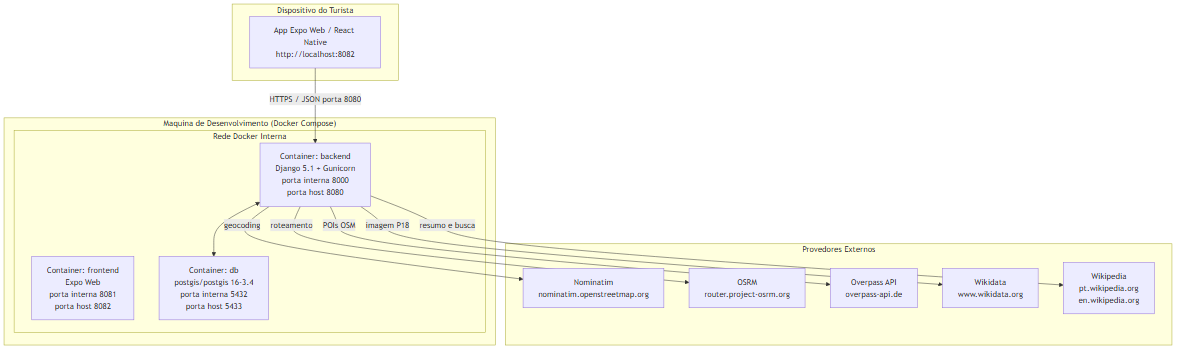
\includegraphics[width=0.85\textwidth]{figuras/implantacao.png}
  \caption{Diagrama de implanta\c{c}\~ao -- ambiente Docker de desenvolvimento}
\end{figure}

O ambiente de desenvolvimento usa Docker Compose com tr\^es containers: \texttt{backend} (Django + Gunicorn, porta 8080), \texttt{frontend} (Expo Web, porta 8082) e \texttt{db} (PostgreSQL + PostGIS, porta 5433) \cite{docker2024}.

\subsection{Modelagem de dados}

\subsubsection{Diagrama Entidade-Relacionamento}

\begin{figure}[H]
  \centering
  
\includegraphics[width=0.95\textwidth]{figuras/er.png}
  \caption{Diagrama ER do Explora+ -- MVP entregue}
\end{figure}

O modelo de dados evoluiu significativamente em rela\c{c}\~ao \`a proposta inicial. A entidade \texttt{Route} de destino \'unico foi substitu\'ida por um conjunto de entidades que suportam rotas multi-POI e personaliza\c{c}\~ao por usu\'ario:

\begin{itemize}
  \item \textbf{Place}: fonte \'unica de verdade de um POI. Campo \texttt{source\_ref} \'e o identificador p\'ublico (\texttt{stop\_id} no contrato HTTP). Campo \texttt{detail\_status} controla o ciclo de enriquecimento progressivo.
  \item \textbf{UserPlaceState}: estado global do usu\'ario em rela\c{c}\~ao a um lugar (visitado, contagens, \'ultima rota em que apareceu).
  \item \textbf{RouteSearchCache}: cache de rota calculada por chave can\^onica (origem + destino). Evita recalcular via Nominatim/OSRM/Overpass a cada requisi\c{c}\~ao.
  \item \textbf{TourRoute}: snapshot relacional da rota personalizada do usu\'ario com geometria LineString PostGIS.
  \item \textbf{TourRouteStop}: cada POI na rota com estado \texttt{active / visited / excluded}.
\end{itemize}

\subsubsection{Diagrama de Classes}

\begin{figure}[H]
  \centering
  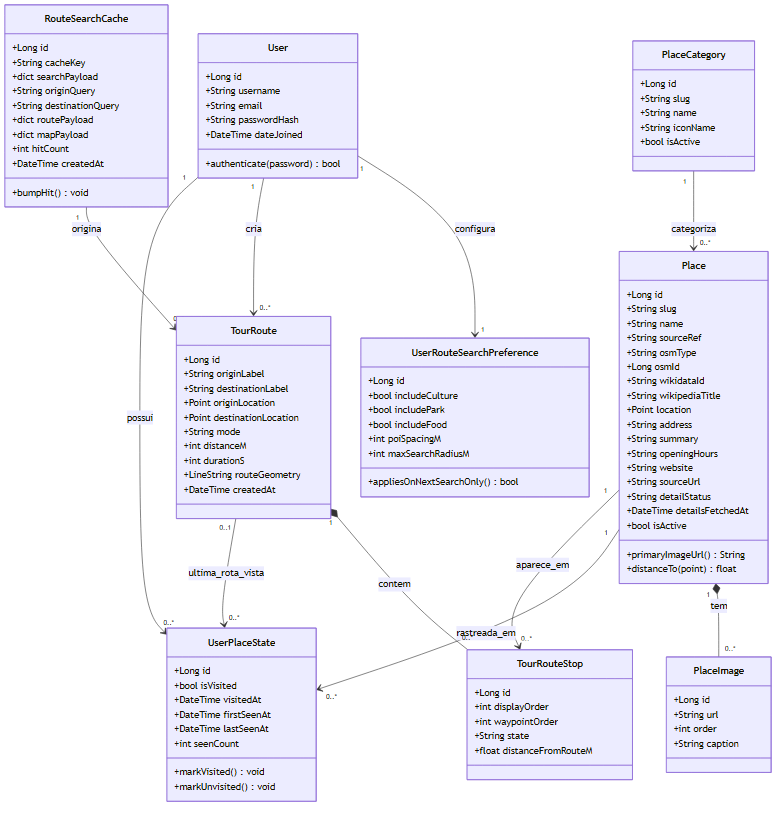
\includegraphics[width=0.95\textwidth]{figuras/classes.png}
  \caption{Diagrama de classes principal}
\end{figure}

\subsection{Casos de Uso}

\begin{figure}[H]
  \centering
  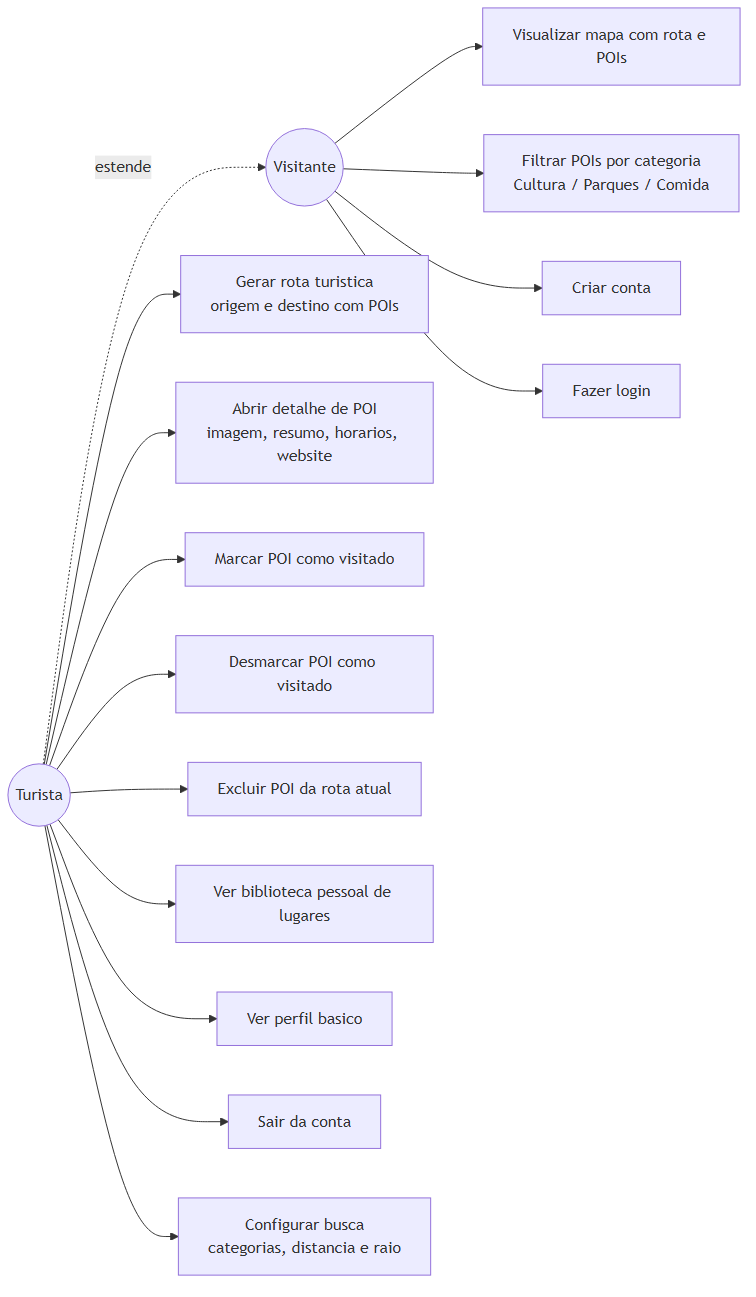
\includegraphics[width=0.85\textwidth]{figuras/casos-de-uso.png}
  \caption{Diagrama de casos de uso -- MVP}
\end{figure}

O MVP define dois atores: \textbf{Visitante} (usu\'ario an\^onimo) e \textbf{Turista} (usu\'ario autenticado, que estende Visitante). O ator Administrador da proposta inicial foi removido do escopo: lugares s\~ao populados via comando \texttt{seed\_demo} e descobertos automaticamente pelo Overpass API.

\subsection{Fluxos principais}

\subsubsection{Gerar Rota Tur\'istica}

\begin{figure}[H]
  \centering
  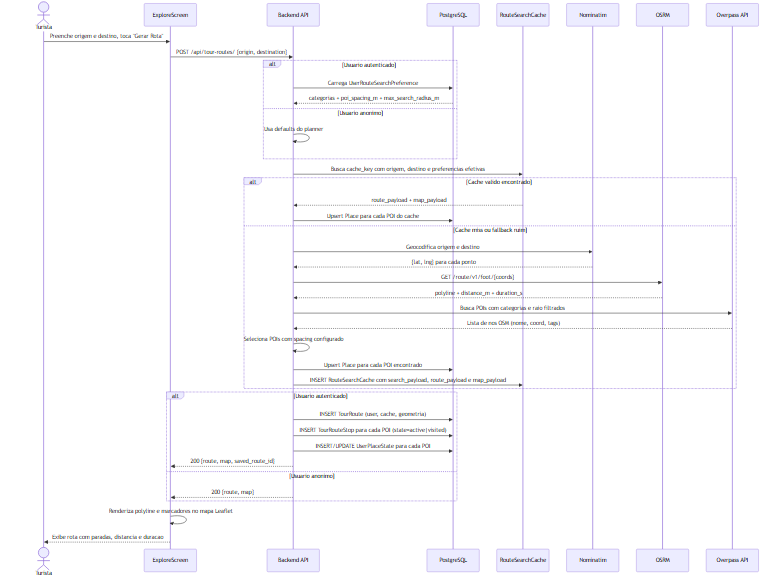
\includegraphics[width=0.95\textwidth]{figuras/sequencia-gerar-rota.png}
  \caption{Diagrama de sequ\^encia -- Gerar Rota}
\end{figure}

O fluxo de gera\c{c}\~ao de rota \'e o n\'ucleo do produto. Ao receber \texttt{POST /api/tour-routes/} com origem e destino, o backend: (1) verifica o cache por chave can\^onica; (2) em caso de miss, geocodifica via Nominatim, calcula rota pedestre via OSRM e busca POIs via Overpass; (3) realiza upsert dos POIs em \texttt{Place}; (4) se o usu\'ario estiver autenticado, persiste \texttt{TourRoute}, \texttt{TourRouteStop} e \texttt{UserPlaceState} \cite{osrm2024, overpass2024}.

\subsubsection{Enriquecimento de Detalhe de POI}

\begin{figure}[H]
  \centering
  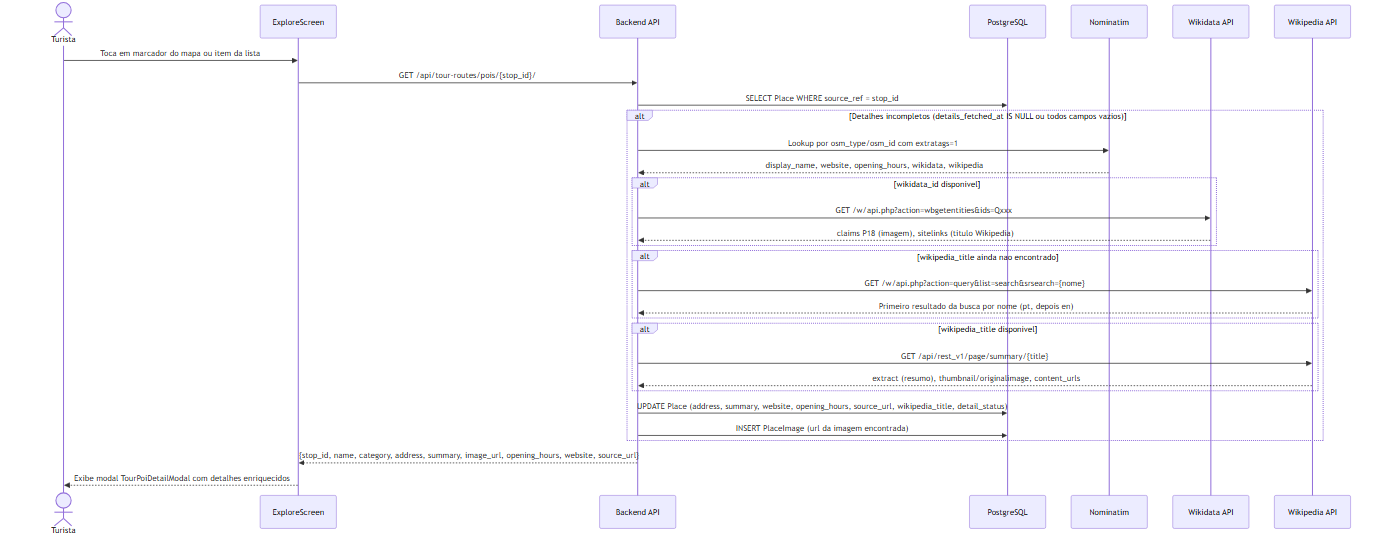
\includegraphics[width=0.95\textwidth]{figuras/sequencia-detalhe-poi.png}
  \caption{Diagrama de sequ\^encia -- Enriquecimento de detalhe de POI}
\end{figure}

Ao abrir o detalhe de um POI (\texttt{GET /api/tour-routes/pois/\{stop\_id\}/}), o backend verifica se os dados j\'a foram enriquecidos. Se n\~ao, executa a cadeia: Nominatim (extratags OSM) $\rightarrow$ Wikidata (imagem P18) $\rightarrow$ Wikipedia por nome (fallback) $\rightarrow$ Wikipedia Summary API.

\subsubsection{Marcar como Visitado}

\begin{figure}[H]
  \centering
  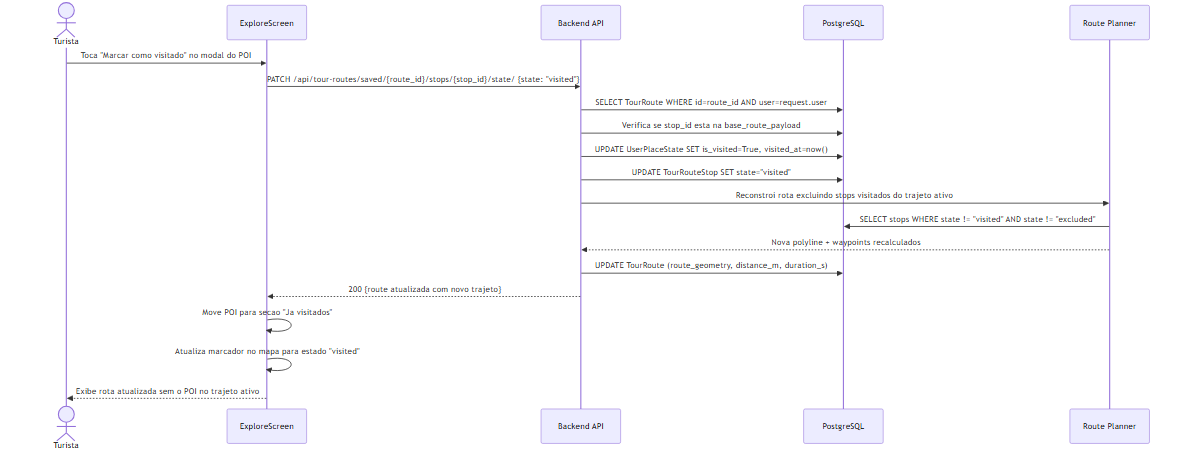
\includegraphics[width=0.85\textwidth]{figuras/sequencia-marcar-visitado.png}
  \caption{Diagrama de sequ\^encia -- Marcar como Visitado}
\end{figure}

Ao marcar um POI como visitado (\texttt{PATCH .../stops/\{stop\_id\}/state/}), o backend atualiza \texttt{UserPlaceState} e \texttt{TourRouteStop}, reconstr\'oi a rota excluindo stops visitados do trajeto ativo, e devolve a rota atualizada.

\subsubsection{Diagrama de Atividade}

\begin{figure}[H]
  \centering
  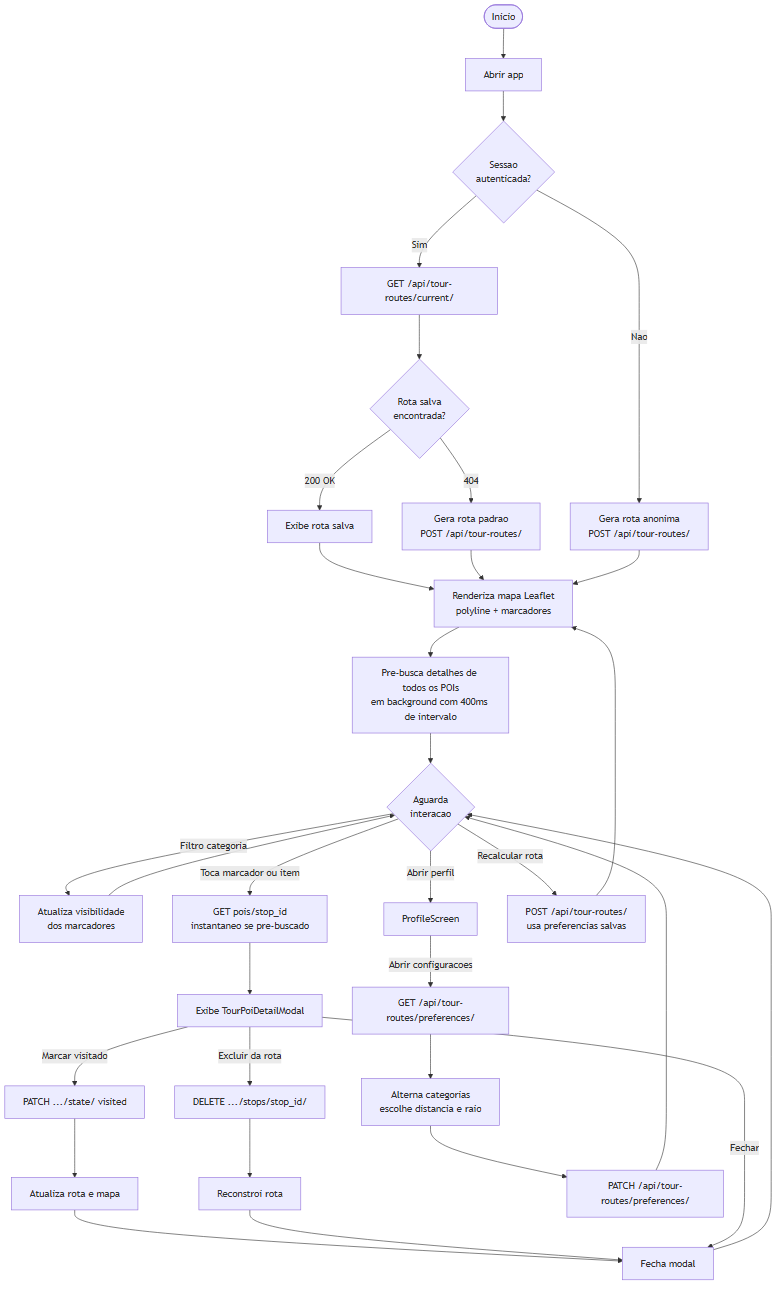
\includegraphics[height=0.82\textheight, keepaspectratio]{figuras/atividade-explorar.png}
  \caption{Diagrama de atividade -- Fluxo da ExploreScreen}
\end{figure}

\clearpage
\subsection{MVP Entregue}

\subsubsection{Funcionalidades implementadas}

\begin{table}[H]
\centering
\caption{Funcionalidades entregues no MVP}
\begin{tabular}{lp{9cm}}
\toprule
\textbf{Funcionalidade} & \textbf{Descri\c{c}\~ao} \\
\midrule
Autentica\c{c}\~ao JWT & Registro, login, refresh de token e logout \\
Planejamento de rota & Origem + destino com POIs selecionados ao longo do percurso \\
Mapa interativo & Leaflet via WebView/iframe com polyline, marcadores e filtros \\
Filtros de categoria & Cultura, Parques, Comida \\
Detalhe de POI & Modal com imagem, resumo, endere\c{c}o, hor\'arios, website \\
Enriquecimento autom\'atico & Imagem e resumo via Wikidata/Wikipedia \\
Marcar visitado & POI sai do trajeto ativo e vai para se\c{c}\~ao ``J\'a visitados'' \\
Excluir POI da rota & Rota recalculada sem o POI exclu\'ido \\
Biblioteca pessoal & Aba Lugares com hist\'orico de todos os POIs vistos em rotas \\
Perfil b\'asico & Dados do usu\'ario e bot\~ao de logout \\
Cache de rotas & Rota reutilizada para mesma origem/destino sem recalcular \\
\bottomrule
\end{tabular}
\end{table}

\subsubsection{Funcionalidades fora do escopo atual}

As seguintes funcionalidades foram identificadas na proposta inicial, mas n\~ao foram implementadas neste ciclo por decis\~ao de escopo:

\begin{itemize}
  \item Integra\c{c}\~ao com eventos culturais (Sympla, TicketMaster);
  \item Integra\c{c}\~ao com aplicativos de mobilidade (Uber, 99);
  \item Consulta de transporte p\'ublico (Quanto Tempo Falta);
  \item Sele\c{c}\~ao de modal de transporte (apenas caminhada suportada);
  \item Compra real de ingressos (endpoint mockado);
  \item Edi\c{c}\~ao de perfil de usu\'ario;
  \item Busca por voz.
\end{itemize}

% -----------------------------------------------------------
\section{Conclus\~ao}
% -----------------------------------------------------------

O Explora+ entregou um MVP funcional e coerente que cumpre o objetivo central do projeto: permitir que turistas e moradores descubram e percorram pontos de interesse em Santos com aux\'ilio de um app m\'ovel.

A principal mudan\c{c}a em rela\c{c}\~ao \`a proposta inicial foi a substitui\c{c}\~ao de APIs comerciais por alternativas abertas (Nominatim, OSRM, Overpass, Wikidata, Wikipedia), o que tornou o sistema mais sustent\'avel e independente de cotas e custos. O modelo de dados evoluiu de uma rota \emph{single-destination} para um planner multi-POI com cache, personaliza\c{c}\~ao por usu\'ario e enriquecimento progressivo de conte\'udo.

\subsection{Justificativas t\'ecnicas das escolhas}

\begin{description}
  \item[React Native + Expo] Gera aplica\c{c}\~ao nativa para Android, iOS e Web a partir de uma \'unica base de c\'odigo, reduzindo custo de manuten\c{c}\~ao \cite{reactnative2024, expo2024}.
  \item[Django + DRF] Maturidade do framework, mapeamento ORM direto das entidades de neg\'ocio e seguran\c{c}a integrada \cite{django2024, drf2024, holovaty2009}.
  \item[PostgreSQL + PostGIS] Suporte nativo a opera\c{c}\~oes geoespaciais (dist\^ancia, proximidade, LineString) necess\'arias para roteamento e sele\c{c}\~ao de POIs \cite{postgis2024}.
  \item[OpenStreetMap + Nominatim + OSRM + Overpass] Alternativa gratuita, global e com cobertura adequada para Santos. Elimina depend\^encia de APIs pagas \cite{osm2024, nominatim2024, osrm2024, overpass2024}.
  \item[Wikidata + Wikipedia] Fonte rica de imagens e descri\c{c}\~oes culturais para pontos de interesse, sem necessidade de curadoria manual \cite{wikidata2024, wikipedia2024}.
  \item[Docker + Docker Compose] Ambiente de desenvolvimento id\^entico para todos os integrantes, com hot reload e isola\c{c}\~ao de depend\^encias \cite{docker2024, humble2010}.
\end{description}

% -----------------------------------------------------------
\printbibliography[title={Refer\^encias}]

\end{document}
